\documentclass[border=3pt]{standalone}
% Preâmbulo compartilhado pelos diagramas TikZ da aula 9 de IHC (Princípios e Diretrizes)
\usepackage[T1]{fontenc}
\usepackage[utf8]{inputenc}
\usepackage{lmodern}
\usepackage{amsmath}
\usepackage{xcolor}
\usepackage{tikz}
\usetikzlibrary{arrows.meta,angles,quotes,decorations.pathmorphing,decorations.pathreplacing,calc,
                positioning,shapes.geometric,shapes.misc,backgrounds,fit,
                math}

% Paleta (mesma dos SVGs originais)
% Paleta da disciplina de IHC: acento roxo (#755099), da capa do livro.
% (o nome "dblue" é mantido para não alterar todos os diagramas)
\definecolor{dblue}{HTML}{755099}
\definecolor{dorange}{HTML}{B3541E}
\definecolor{dgreen}{HTML}{4A7C59}
\definecolor{dred}{HTML}{9C4B4B}
\definecolor{dcream}{HTML}{F4F1EA}
\definecolor{dshade}{HTML}{DDD7C9}

% Função gaussiana (não normalizada por padrão de escala visual)
\pgfmathdeclarefunction{gauss}{3}{%
  \pgfmathparse{1/(#3*sqrt(2*pi))*exp(-((#1-#2)^2)/(2*#3^2))}%
}

% Estilos comuns (prefixo d... para não colidir com chaves internas do pgf)
\tikzset{
  >={Stealth[length=2mm]},
  dguide/.style={gray!55, dashed, line width=0.4pt},
  daxis/.style={gray!60, line width=0.7pt, ->},
  dbody/.style={fill=black!3, draw=black!80, line width=1pt},
  dacc/.style={draw=dblue, line width=1pt},
  dlbl/.style={black!55, font=\small},
  dsub/.style={black!45, font=\footnotesize},
  dstate/.style={circle, draw=black!80, fill=dcream, line width=1pt,
                 minimum size=17mm, font=\large, inner sep=1pt},
  dobs/.style={circle, draw=black!80, fill=dshade, line width=1pt,
               minimum size=14mm, font=\large, inner sep=1pt},
  dbox/.style={rounded corners=2pt, draw=black!80, fill=dcream, line width=1pt,
               align=center, inner sep=6pt},
  dop/.style={circle, draw=black!80, fill=white, line width=1pt,
              minimum size=6mm, inner sep=0pt, font=\small},
  dtrans/.style={->, dblue, line width=1pt},
  dmeas/.style={->, dorange, line width=1pt},
  dcurve/.style={line width=1pt, dblue},
  dcurveb/.style={line width=1.4pt, dorange},
}

\begin{document}
\hyphenpenalty=10000 \exhyphenpenalty=10000 \tolerance=9999 \emergencystretch=3em
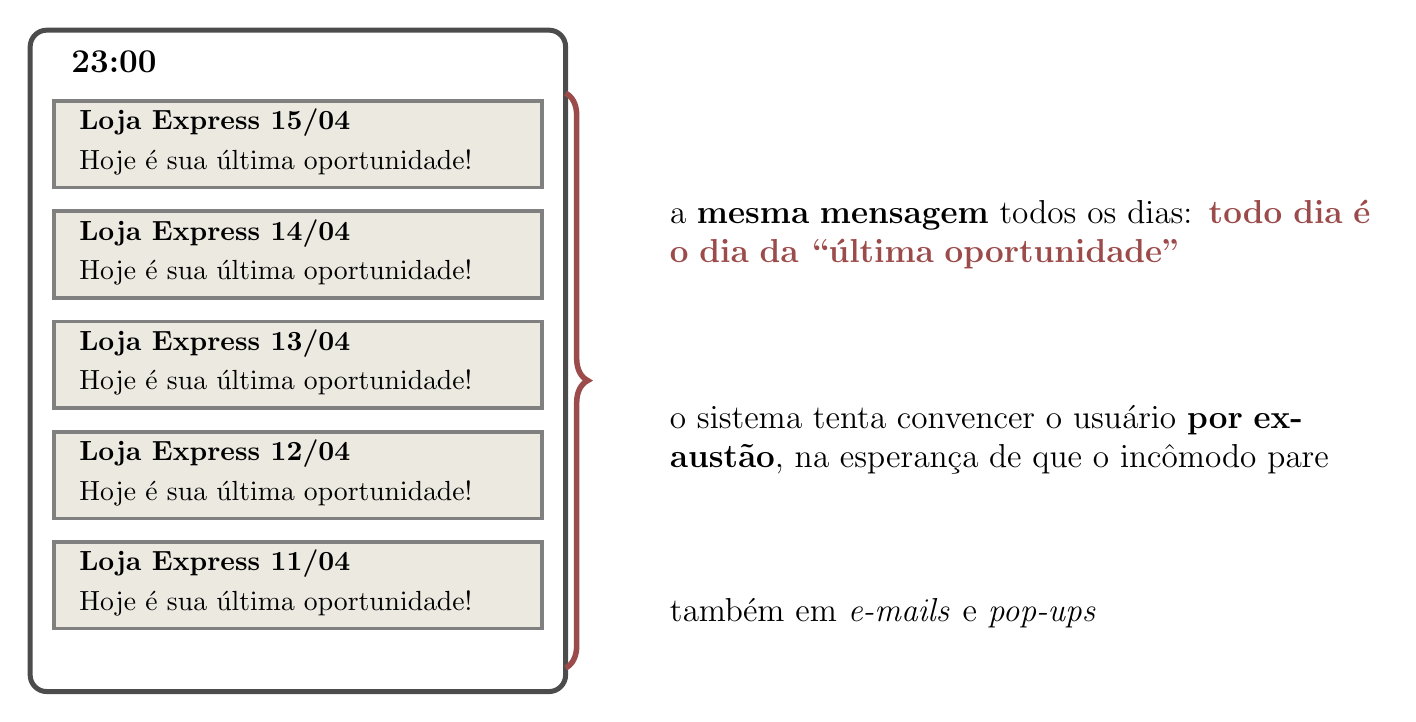
\begin{tikzpicture}[x=1cm,y=1cm]
\draw[draw=black!70, line width=1.8pt, fill=white, rounded corners=6pt] (0,0) rectangle (6.8,8.4);
\node[font=\large\bfseries, anchor=west] at (0.4,8.0) {23:00};
\foreach \i/\d in {0/{15/04}, 1/{14/04}, 2/{13/04}, 3/{12/04}, 4/{11/04}} {
  \draw[draw=black!50, line width=1.3pt, fill=dshade!55] (0.3,{6.4-\i*1.4}) rectangle (6.5,{7.5-\i*1.4});
  \node[font=\normalsize\bfseries, anchor=west] at (0.5,{7.22-\i*1.4}) {Loja Express \d};
  \node[font=\normalsize, anchor=west] at (0.5,{6.72-\i*1.4}) {Hoje é sua última oportunidade!};}
\draw[decorate, decoration={brace, amplitude=8pt, mirror}, line width=2pt, dred] (6.8,0.3) -- (6.8,7.6);
\node[font=\large, anchor=west, text width=9cm] at (8.0,5.8) {a \textbf{mesma mensagem} todos os dias: \textbf{\textcolor{dred}{todo dia é o dia da ``última oportunidade''}}};
\node[font=\large, anchor=west, text width=9cm] at (8.0,3.2) {o sistema tenta convencer o usuário \textbf{por exaustão}, na esperança de que o incômodo pare};
\node[font=\large, anchor=west, text width=9cm] at (8.0,1.0) {também em \emph{e-mails} e \emph{pop-ups}};
\end{tikzpicture}
\end{document}
